%% Thesis template
%% PMC, University of Minho
%% if required, comment unused packages
\documentclass[12pt,english,oneside]{book}
% \usepackage[portuguese]{babel}
% \usepackage[utf8]{inputenc} 
\usepackage{times}
\usepackage[T1]{fontenc}
\usepackage[latin1]{inputenc}
\usepackage{a4wide}
\usepackage{fancyhdr}
\pagestyle{fancy}
\usepackage{subfigure}
\usepackage{float}
\usepackage{graphicx}
\usepackage{setspace}
\usepackage{algpseudocode}
\usepackage{varwidth}
\usepackage{caption}
\usepackage{cite}\onehalfspacing



\makeatletter

%%%%%%%%%%%%%%%%%%%%%%%%%%%%%% LyX specific LaTeX commands.
%% Bold symbol macro for standard LaTeX users
\newcommand{\boldsymbol}[1]{\mbox{\boldmath $#1$}}

\floatstyle{ruled}
\newfloat{algorithm}{tbp}{loa}
\floatname{algorithm}{Algorithm}

%%%%%%%%%%%%%%%%%%%%%%%%%%%%%% Textclass specific LaTeX commands.
 \usepackage{verbatim}
 \newenvironment{lyxlist}[1]
   {\begin{list}{}
     {\settowidth{\labelwidth}{#1}
      \setlength{\leftmargin}{\labelwidth}
      \addtolength{\leftmargin}{\labelsep}
      \renewcommand{\makelabel}[1]{##1\hfil}}}
   {\end{list}}

%%%%%%%%%%%%%%%%%%%%%%%%%%%%%% User specified LaTeX commands.
\usepackage{color}
\usepackage{colortbl}
\usepackage{url}
\input{epsf}
\newcommand{\single}{\renewcommand\baselinestretch{1.0}}
\newcommand{\onehalf}{\renewcommand\baselinestretch{1.5}}
\newcommand{\double}{\renewcommand\baselinestretch{2.0}}
\fancyhead{}
\fancyhead[LE]{\slshape \leftmark}
\fancyhead[RO]{\slshape \rightmark}
\cfoot{\thepage}
\setlength{\parskip}{2mm}

\usepackage{babel}
\makeatother
\begin{document}
\begin{minipage}[c]{1.0\columnwidth}%
\begin{doublespace}
\vspace{2cm}
\begin{center}{\huge A new Framework to enable rapid innovation in Cloud Datacenter through a SDN approach.}\end{center}{\huge \par}
\end{doublespace}

\vspace{2cm}
\begin{center}{\large Jos\'{e} Teixeira}\end{center}{\large \par}
\vspace{2cm}

\begin{quote}
\begin{center}A thesis submitted to the University of Minho in the
subject of Informatics, for the degree of
% or Doctor of Philosophy 
Master of Science, under scientific supervision of Prof. Stefano Giordano and Prof. Alexandre Santos\end{center}\vspace{3cm}

\end{quote}
\begin{singlespace}
\begin{center}University of Minho\end{center}

\begin{center}School of Engineering\end{center}

\begin{center}Department of Informatics\end{center}
\end{singlespace}

\begin{center}{\large September, 2013}\end{center}\end{minipage}%
\thispagestyle{empty}

\pagenumbering{roman}


\newpage


\chapter*{Acknowledgments}

\addcontentsline{toc}{chapter}{Acknowledgments}

\noindent I would like...

\medskip{}
\noindent I also...

\chapter*{Abstract}

\addcontentsline{toc}{chapter}{Abstract}

\begin{singlespace}
\hspace{0.6cm}
In the last years, the widespread of Cloud computing as the main paradigm to deliver a large plethora of virtualized services significantly increased the complexity of Datacenters management and raised new performance issues for the intra-Datacenter network.
Providing heterogeneous services and satisfying users' experience is really challenging for Cloud service providers, since system (IT resources) and network administration functions are definitely separated.

As the Software Defined Networking (SDN) approach seems to be a promising way to address innovation in Datacenters, the thesis presents a new framework that allows to develop and test new OpenFlow--based controllers for Cloud Datacenters.
More specifically, the framework enhances both Mininet (a well--known SDN emulator) and POX (a Openflow controller written in python), with all the extensions necessary to experiment novel control and management strategies of IT and network resources.

... talk about obtained results and conclusions(not finished yet, complete when you finish everything)

\end{singlespace}

\paragraph{Keywords:}
Datacenter, Cloud, SDN, OpenFlow.

\newpage

\addcontentsline{toc}{chapter}{Contents}\tableofcontents{}

\clearpage

\chapter*{List of Acronyms}

\addcontentsline{toc}{chapter}{List of Acronyms}

\markboth{LIST OF ACRONYMS}{LIST OF ACRONYMS}

\begin{lyxlist}{00.00.0000}
\begin{singlespace}
\item [DC]Datacenter
\item [DCN]Datacenter Networks
\item [IP]Internet Protocol 
\item [IT]Information Technology
\item [OF]Openflow
\item [QoS] Quality of Service
\item [QoE] Quality of Experience
\item [SDN]Software Defined Networking
\item [VM]Virtual Machine
\item [VMM]Virtual Machine Manager
\item [WAN] Wide Area Network
\item Add as needed...
\end{singlespace}
\end{lyxlist}


\addcontentsline{toc}{chapter}{List of Figures}\listoffigures


\addcontentsline{toc}{chapter}{List of Tables}\listoftables


\setcounter{page}{0}

\pagenumbering{arabic}


\chapter{Introduction\label{cha:introduction}}

\section{Introduction}
\hspace{0.6cm}

A Cloud DC consists of virtualized resources that are dynamically allocated, in a seamless and automatic way, to a plethora of heterogeneous applications.
In Cloud DCs, services are no more tightly bounded to physical servers, as occurred in traditional DCs, but are provided by Virtual Machines that can migrate from a physical server to another increasing both scalability and reliability.
Software virtualization technologies allow a better usage of DC resources; DC management, however, becomes much more difficult, due to the strict separation between systems (\textit{i.e.}, server, VMs and virtual switches) and network (\textit{i.e.}, physical switches) administration.

Moreover, new issues arise, such as isolation and connectivity of VMs.
Services performance may suffer from the fragmentation of resources as well as the rigidity and the constraints imposed by the intra-DC network architecture (usually a multilayer 2-tier or 3-tier fat-tree composed of Edge, Aggregation and Core switches\cite{dc_arch}).
Therefore, Cloud service providers (\textit{e.g.},\cite{amazon}) ask for a next generation of intra-DC networks meeting the following features: 1) efficiency, \textit{i.e.}, high server utilization; 2) agility, \textit{i.e.}, fast network response to server/VMs provisioning; 3) scalability, \textit{i.e.}, consolidation and migration of VMs based on applications' requirements; 4) simplicity, \textit{i.e.}, performing all those tasks easily\cite{baldonado}.

In this scenario, a recent approach to programmable networks (\textit{i.e.}, Software-Defined Networking) seems to be a promising way to satisfy DC network requirements\cite{ibmnec}. 
Unlike the classic approach where network devices forward traffic according to the adjacent devices, SDN is a new network paradigm that decouples routing decisions (control plane) from the traffic forwarding (data plane). This routing decisions are made by a programmable centralized intelligence called controller that helps make this architecture more dynamic, automated and manageable.

Following the SDN--based architecture the most deployed SDN protocol is OpenFlow\cite{openflow}\cite{onf}, and it is the open standard protocol to communicate and control OF-compliant network devices.
Openflow allows a controller to install into OF--compliant network devices forwarding rules which are defined by the administrator/network engineer and match specific traffic flows.

Since SDN allows to re-define and re-configure network functionalities, the basic idea is to introduce an SDN-cloud-DC controller that enables a more efficient, agile, scalable and simple use of both VMs and network resources.
Nevertheless, before deploying the novel architectural solutions, huge test campaigns must be performed in experimental environments reproducing a real DC.
To this aim, a novel framework is introduced that allows to develop and assess novel SDN-Cloud-DC controllers, and to compare the performance of control and management strategies jointly considering both IT and network resources\cite{im2013}.

TODO:should describe better openflow and SDN
% \begin{quote}''OpenFlow allows, for the first time, an external control plane to abstract the entire underlying network fabric so that fabric is universally addressable and all topology and state information is commonly managed''{ --- \textup{ Jason Matlof}, vice president of marketing at Big Switch}\end{quote}

% \newpage
\section{Motivation and objectives\label{sec:motobj}}
\hspace{0.6cm}

Although SDN came as a solution to fulfill the network requirements of the DCs, the only point of interaction with the IT resources is the generated traffic.
By definition SDN does not go further, but if there could be a controller that manages both IT and network resources, all the information could be shared easily and both of them could greatly benefit: the network could start to anticipate IT actions and adapt itself to have higher performance, more redundancy, etc; the IT because the resources could be better managed so that the network, not only stops being the bottleneck, but actually helps the IT complete the tasks faster and without affecting adjacent resources.

When developing an Openflow controller, the administrator/network engineer goals are to implement the desired behaviour and to test it (making sure it suits the requirements).
The currently available controllers already provide some abstraction, which varies according to the type of programming language, but they are still too low level to allow rapid innovation. 
Following the implementation, tests campaigns must be performed and for it a controlled environment should be set.
Although Openflow allows the use of slices of the real network for testing purposes, it is more convenient to use an emulator since the DC size can be dynamic, different scenarios can be easily produced and it only needs a single computer -- Mininet is such an emulator.
Despite its flexible API, Mininet does not provide any type of traffic generator and is not DC--oriented: poor topology generation regarding DCs; no support for VMs;

A whole framework composed by a modified OF controller that allows the access to both IT and network resources through an easy-to-use but full featured API, and a testing environment that communicates with it to provide a real DC emulation is the the main objective.
With this is is expected to endue the administrator/network engineer with all the tools needed to quickly develop, test and deploy VM and network management strategies into a DC.

% When the admin wants to try new DC VM allocation algorithms, first it takes to long to develop since the current controllers are still low level, and second if they want to test, or they try on their own DC (which could compromise the normal functioning and unless they try on a small part of the DC the result wont be accurate since they would be influences by the usual workload.
% Or they would use simulators(the problem with simulator is that usually you have to rewrite the algorithms that you will implement, and the results might not be accurate (correspond to the real environment)).
% At the same time, a whole framework that provides support to develop and test only the logic that the admin wants would also be cool, since they could focus on making new VM allocations that consider multiple factor (this is where OF helps since it has info about network)
% Maybe also talk a little about allowing to be easily expandable, extended.

% \begin{itemize}
% 	\item Understanding the basic features of SDN paradigm
% 	\item Studying the problematics in cloud DC VM allocations
% 	\item Apply the SDN paradigm to better exploit the DC resources
% 	\item Develop a framework for Cloud Datacenter emulation and new VM allocation policies
% 	\item ...
% \end{itemize}


\section{Thesis layout}
\hspace{0.6cm}

This thesis is structured into five chapters: the present Chapter \ref{cha:introduction} is a brief introduction of the proposed work, its motivation and objectives; the second is the state of art, it addresses the currently available solutions relating innovation in DCs, OF controllers and VM allocation and migration algorithms; the third one fully describes the framework, its evolution, extensions and how it can be used; in the forth chapter is presented the framework validation and performance tests; and in the last chapter are made conclusions about the developed work, as well as suggestions for future work.



\chapter{State of art \label{cha:stateofart} }

\section{Available solutions}

A number of research efforts have focused on novel solutions for emulation/simulation of Cloud DCs.
The available solutions provide a reference and material to analise and explore the concepts addressed along this thesis. 
This section presents and overview of them, highlighting their architecture, features and limitations.

\subsection{CloudSim}
\hspace{0.6cm}

Calheiros et al.\cite{cloudsim} proposed a Java-based platform, called Cloudsim, that allows to estimate cloud servers performance using a workflow model to simulate applications behaviour.
By providing a framework for managing most key aspect of a Cloud infrastructure (DC hardware and software, VM placement algorithm, Applications for VM, Storage access, Bandwidth provisioning) and by taking into consideration factors as energy-aware computational resources and costs, it helps to identify possible bottlenecks and improve overall efficiency.

Regarding the network aspect of Clousim, Garg et al.\cite{cloudsim2} extended such a system with both a new intra--DC network topology generator and a flow--based approach for collecting the value of network latency. However, in such a simulator, networks are considered only to introduce delay, therefore it is not possible to calculate other parameters (\textit{e.g.}, Jitter).
A SDN extension for Cloudsim as already been thought, Kumar et al.\cite{cloudsim3}, but it still just an architecture design, meaning it has not been implemented yet.

Although it allows to predict how the management strategies will behave, as a simulator, it does not allow to run real applications and deploying the tested management logic in a real environment still requires everything to be developed.

\subsection{FPGA Emulation}
\hspace{0.6cm}

Ellithorpe et al.\cite{box} proposed, a FPGA emulation platform that allows to emulate up-to 256 network nodes on a single chip.
\begin{quotation}
''Our basic approach to emulation involves constructing a model of the target architecture by composing simplified hardware models
of key datacenter building blocks, including switches, routers, links, and servers. Since models in our system are implemented in programmable hardware, designers have full control over emulated buffer sizes, line rates, topologies, and many other network properties.''

\hfill Ellithorpe et al.\cite{box}
\end{quotation}

This platform also allows the emulation of full SPARC v8 ISA compatible processor, which along with full system control provides a greater system visibility.
However, hardware programming skills might be a requirement and the cost of a single board is approximately 2, 000 dollars making this solution less attractive than ones based on just open--source software.

\subsection{Meridian}
\hspace{0.6cm}

Following the new shiny SDN paradigm, Banikazemi et al.\cite{meridian} proposed Meridian, an SDN--based controller
framework for cloud services in real environments.

\begin{figure}[htbp]
        \centering
        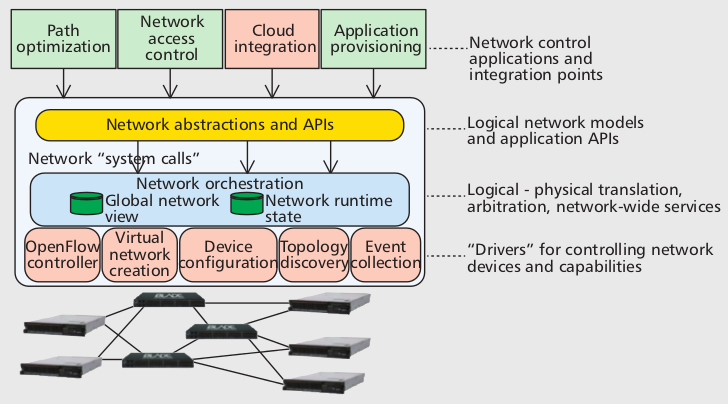
\includegraphics[width=0.8\textwidth]{figures/meridian_arch.png}
        \caption{Meridian SDN cloud networking platform architecture (Banikazemi et al.\cite{meridian})}
        \label{fig:meridian_arch}
\end{figure}

As shown in figure \ref{fig:meridian_arch}, the architecture is divided into three main layers: Network abstractions and API, where the network information can be accessed and manipulated (\textit{e.g.} access controlling policies, prioritizing traffic); Network Orchestration, translates the command provided by the API into physical network commands and orchestrates them for more complex operations. it also reveals the network topology and its variations; finally the ''drivers'' layer is an interface for underlying the network devices so several network devices and tools can be used.

Generally, this platform allows to create and manage different kind of logical network topologies and use their information for providing a greater control of the DC.
But as it works on top of a cloud Iaas platform (i.e., Openstack\cite{openstack}, IBM SmartCloud Provisioning\cite{scp}), it is limited to their management strategies and is only useful if one already has this type of infrastructure. Not having a testing environment is also a downside since the normal operation can be compromised and also alter the testing results.

\subsection{ICanCloud, GreenCloud and GroudSim}
\hspace{0.6cm}

Other well--known open--source cloud simulators are ICancloud\cite{icancloud}, GreenCloud\cite{greencloud} and GroudSim\cite{groudsim}, but in none of them SDN features are available.

\newpage
\subsection{Mininet}
\hspace{0.6cm}
\begin{quotation}

''Mininet is a network emulator which creates a network of virtual hosts, switches, controllers, and links. Mininet hosts run standard Linux network software, and its switches support OpenFlow for highly flexible custom routing and Software-Defined Networking.''

\hfill Mininet \cite{mininet}
\end{quotation}

As a network emulator for SDN systems, mininet can generate OF compliant networks that connect to real controllers without the need of hardware resources. Such features derives from the use of Open vSwitch and enables the assessment of the operation of an OF controller before its deployment in a real environment.

It also provides tools for automatically generating topologies, however, as they can be basic, an API is available to reproduce any type of topology and experiments.
Mininet hosts behave just like real hosts, can run any program as long as it does not depend on non linux kernels, and can send packets through emulated interfaces.
But as they share the same host file system and PID space, a special attention is required when killing/running programs.

Despite its flexibility, Mininet lacks of a complete set of tools that easily allow to emulate the behaviour of a cloud DC, thus raising the following questions:
 
\begin{itemize}
\item How to easily generate and configure typical DC topologies?
\item How to simulate VMs allocation requests?
\item How to emulate the inter and in/out DC traffic?
\end{itemize}

\newpage
\section{Openflow Controllers}
\hspace{0.6cm}


\newpage
\section{Virtualization Platforms}
\hspace{0.6cm}
% Uncomment to include file.pdf
%\begin{figure}%[H]
%\begin{center}\includegraphics[scale=0.8]{file}\end{center}
%\caption{Legend \label{fig:LABEL}}
%\end{figure}


\chapter{The Framework \label{cha:framework} }


\section{Requirements}
\hspace{0.6cm}

Provide the user with a full package for the development and test of DC SDN Controller was one of the main purposes of the framework.
Aiming for such goal, but without discarding the deployment in a real DC, a single software platform was designed and developed.
Because the requirements change according to the controller being in the development or the deployment phase, so should the platform by creating and environment that best suits each of them.

\paragraph{Development \& Testing Phase}
\hspace{0.6cm}

Encourage a rapid development is one of the main requirements since it promotes innovation in the cloud DC.
It must be simple and fast to develop the desired logic, which can be achieved by providing easy access to information and management of the network and servers.
More specifically, automatic topology detection (and changes in it) associated with a high level API for accessing and managing switch's and server's information and statistics.

When testing, the framework should provide an automatic way of generating the VM requests and the traffic associated to each request (for testing the VM allocation and the network behaviour).
The traffic generator should also correctly represent the DC traffic profiles.
Allowing an easy access outside the controller for the statistics is also important, so it is possible to analyze the logic effects on the DC.

\paragraph{Deployment Phase}
\hspace{0.6cm}

For the deployment, the framework should be easy to configure and monitor, and no extra effort should be made for the framework to run on the real DC (it should adapt automatically). There should also be an intuitive way to make manual VM requests, so clients can generate and manage their own VMs.

\section{Chosen technologies}

\subsubsection{Openflow Controller: POX}
\hspace{0.6cm}

Being POX a python derivative of the NOX controller, which was developed by the same people who developed the Openflow protocol, adopting it would be a surplus since there is a higher chance it will continue to support Openflow, and that the new versions/features are available as soon as possible.
Besides, being a high level (comparing to C and C++), object and event oriented programming language, helps to create the abstraction level required for agile development and turn the controller more interactive.

\subsubsection{Datacenter Emulator: Mininet}
\hspace{0.6cm}

Mininet comes recommended in the Openflow tutorials as the platform for testing the OF compliant controllers.
It also provides an API in python for the development of custom made topologies and specific experiments, which along with the capacity that the virtualized hosts have of running almost any program, makes it a powerful platform.

\subsubsection{Virtualization platform: XCP 1.6 (Xen Cloud Platform)}
\hspace{0.6cm}

As a free and opensource platform though for the cloud, XCP bring all the features belonging to Xen, plus it comes with ready-to-install images, making it simpler to install and configure.
Having multiple interaction option is also an attractive feature, but having a Xen python API was decisive since hit gave the possibility to write all the code in one programming language which helps keeping the platform consistent.
\newpage

\section{Framework architecture}
\hspace{0.6cm}

\begin{figure}[htbp]
        \centering
        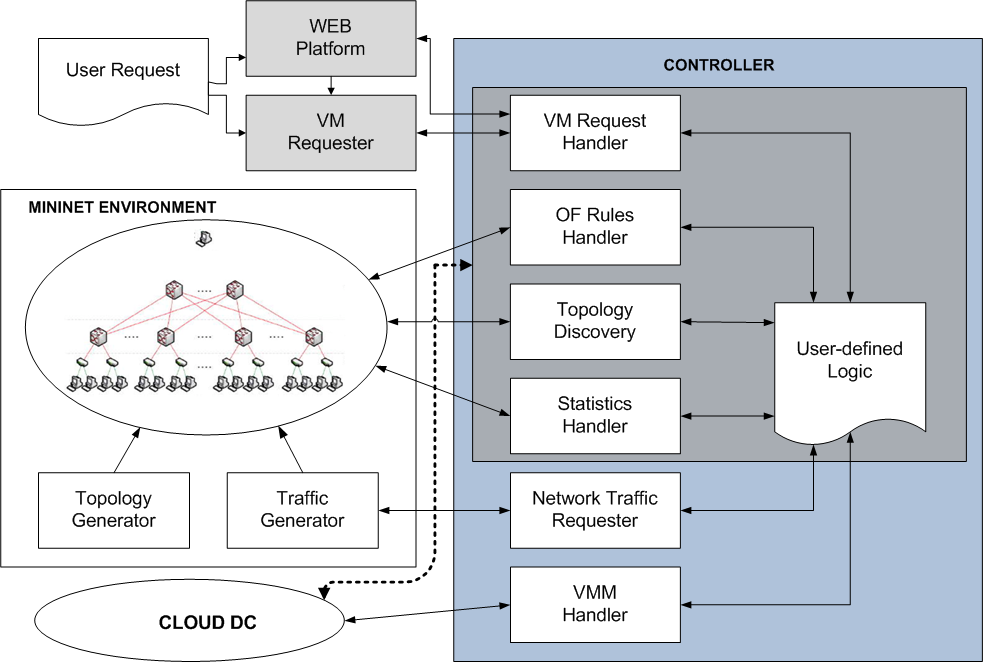
\includegraphics[width=0.8\textwidth]{figures/emulator_new.png}
        \caption{Framework Architecture}
        \label{fig:framework}
\end{figure}

The framework architecture, shown in figure \ref{fig:framework}, gives an overview of the its modules and their interaction.
The framework is divided into two main parts: the mininet environment - an extended version of mininet; and the controller - a modified, improved version of POX;

The mininet environment is made to be only used when testing the controller.
It is composed by the mininet platform with two extra modules that explore its API.
One of them is the {\it Topology Generator}, which allows to easily create multilayer 2-tier or 3-tier fat-tree DC topologies.
The other one is the {\it Traffic Generator} that allows to correctly simulate the allocation of VM into each server by generating traffic from that server to the exterior of the DC. It also allows to simulate inter VM communication.

As for the controller, it automatically manages the modules in order to only use the ones that are needed for each phase (development and testing or deployment).
Depending on it, the controller will interact with the mininet environment or the Cloud DC, which represents the real Cloud DC infrastructure.
In the figure \ref{fig:framework}, in the controller part, it can be seen a darker area which corresponds to the modules that are used in both phases. These modules are:
\begin{itemize}
  \item VM Request Handler -- Connects with the Web platform and/or the VM requester, and processes the VM requests;
  \item OF Rules Handler -- Manages and keeps track of the installation/removal of the OF rules from the switches;
  \item Topology Discover -- Manages all the information regarding the switches, links, servers and its detection;
  \item Statistics Handler -- Collects statistics about the switches and links. Can be periodical or manual;
  \item User-defined Logic -- Space for the administrator/network engineer to develop the desired DC management logic;
\end{itemize}

Regarding the other controller modules: the {\it Network Traffic Requester} which is only used when performing tests, tells the mininet environment how much, when, from where and where to, the traffic should be generated; and the {\it VMM Handler} which is only active when the controller is in a real environment, communicates with the hypervisor to perform all the operations regarding the VMs (allocate, deallocate, upgrade, etc).

Outside of the the mininet environment and the controller there is the {\it WEB platform} and the {\it VM Requester}, that where created for making VM requests. While the first one is a platform where DC clients can request (and manage) VMs that will be processed by the controller and later allocated by the hypervisor (oriented for the deployment phase), the {\it VM Requester} is an automatic full configurable VM request generator powered by random variables (oriented for the testing phase).

An important feature that was taken into consideration when designing the framework's architecture is that all the modules are independent from each other, and they can be changed, removed or added in order to fulfill all the user requirements.

\section{Directory structure}

-also explain that it was an evolving process, and it was change to make it easier to understand
Explain the directory /file structure and how it maps to the architecture

\section{Framework modules: Mininet Environment}

Describe each module, it's functionalities, limitations, how it can be used/improved (improved if the user wants to add new features)

Talk about the configuration file

\subsection{Topology Generator}

Mininet predefined topology generator only have tree topologies and they don't have a Gateway, so after traffic reaches the core switches it goes nowhere (if it is traffic that addresses the internet).

As so, using the API it was generated a costume topology.
-allows to choose the number of edge,agg and core switches,
- how many connection exist between them. (links are created automatically)
-number of servers also and how much edge switches does each of them connects
-same thing for the DC gateways with the core switches
-links bandwidth can be chosen for each link category
-everything can be configured by the configuration file, so it's easy to create different cenarious

\subsection{Traffic Generator}
\hspace{0.6cm}

Talk about the first approach:
-Use tcpreplay with a DC traffic sample
-Modify the sample to suit each server
-Use server/client for ordering the starting of the traffic
-play it at the requested speed from the servers that got the vm allocation
-problems found: Samples must be generated with the corrrect ip addresses (takes time), short term solution was generate them previously for all the possible servers, so they can be just reproduced when ask (instead of waiting)
-problems found: tcpreplay takes to much cpu independently of the amount of traffic that is generated
-"amostra" de tráfego do cluster do DI com 500mb


Talk about the Iperf solution
-able to generate UDP and TCP traffic
-although is not accurate to "imitate" DC traffic behaviour, it is good for testing the DC limits and how it behaves when is overloaded, or near overloading
-doesn't have the problem that tcp replay had
-included possible configuration in the configuration file for simplicity

Talk about d-itg:
-doesnt have the problem Tcpreplay has
-its much more dynamic then iperf (allows to generate voip,...)

\newpage

\section{Framework modules: Controller}
\hspace{0.6cm}

Describe each module, it's functionalities, limitations, how it can be used/improved (improved if the user wants to add new features)

Talk about the configuration file, and talk about how it was before (interactive parametrization (consoles asks for info), if no config file exists, it can be created this way)

\subsection{Topology}
\hspace{0.6cm}

-saves all the info regarding topology (switches, hosts(servers or gateways(NOTE: non OF switches are viewed as hosts)), their interfaces, and the links)
-saved in disctionaries for easy and fast access to information
-responsible for discovering the topology and update the information acording to the changes that occur.
-explain how topology is discovered and which modules are used (Pox discovery which uses lldp packets and host\_tracker which uses ping (i guess, check it))
-explain how host tracker was modified and which events where added
-explain to which event it listens and what does it do with them.

\subsection{Rules (OF Rules Handler)}
\hspace{0.6cm}

-Saves info about the rules that were installed on each switch
-install/deletes rules as VMs are install /expire
-routing is defined by user, this modules just provides abstraction for the lower level methods provided by pox.
-methods based only on dest and source ip, and more complex methods for higher traffic control.
Future work:
-aggregate rules?
-suppernetting?
-show information in webplatform (for admin and allow admin to override controller actions (change routes, shutdown links, etc))

\subsection{Stats (Statistics Handler)}

\subsubsection{Statistics}
\hspace{0.6cm}

\begin{figure}[h!tbp]
\centering
\begin{minipage}{.5\textwidth}
  \centering
  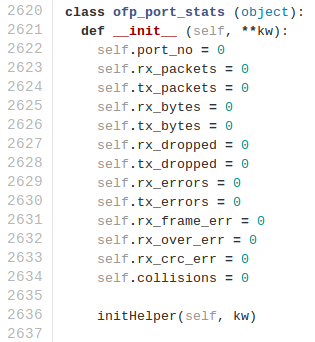
\includegraphics[width=0.8\textwidth]{figures/stats_portstats.png}
  \caption{Available port statistics}
  \label{fig:stats_portstats}
\end{minipage}%
\begin{minipage}{.5\textwidth}
  \centering
  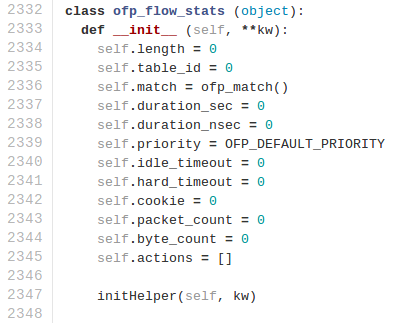
\includegraphics[width=1\textwidth]{figures/stats_flowstats.png}
  \caption{Available flow statistics}
  \label{fig:stats_flowstats}
\end{minipage}%
\end{figure}

In figure \ref{fig:stats_portstats}, it can be seen all the statistics available for switch ports and flows.

-explain the statistics available
-say there is no bitrate, and since it is an important one (and modifying OF protocols was not a good option) we opted by calculating the bitrate based on the time and the packet count (that's the definition of bitrate, but our approach is not 100\% accurate) (explain how it works)
-talk about the algorithm used for showing the statistics (so its not so reactive, it was adopted a mecanism similar to the one used bu the tcp to calculate the windows size, historical ponderation can be also configured in the configuration file)
-statistics can be retrieved periodically (the peridiodicity is indicated by the configuration file), or can be retrieved whenever is required (for example when a vm request arrives)

-maybe talk about the strcuture in which they are saved and which methods are given for accessing them. 

-Switch/Link ratio
-Switch/link ratio with safe margin (for newer allocation) (configurable by the configuration file - allow over proviioning)


\subsubsection{Statistics Exporter}
\hspace{0.6cm}

For now the Statistics exporter is just saving the values collected into '.csv' files. Two files are generated: one for switches and one for links.
-where the files are placed can be chosen in the configuration file.
-show an example of a file about the bitrate.

Future work:
Export the data into the webplatform.

\subsection{VM Request Handler}
\hspace{0.6cm}

-Explain how it works (by threads and raising events)
-Explain what it does:
  -receives VM requests (process them - make sure they are valid)
  -raise and event saying there is a new VM request
  -waits doe event saying the VM as been allocated or rejected
  -notifies about the state of the request

\subsection{Network Traffic Requester}
\hspace{0.6cm}

-when receives the event wich says the vm as been allocated, it checks if the its is connected to mininet, and if ti is, send a request saying which type of traffic (in case of D-itg - since the type of VM may request the traffic to be of some specific type). In case of iperf, just say the amount of bandwidth.

\subsection{VMM - Virtual Machines Manager}
\hspace{0.6cm}

When the algortithm for choosing the server ends, the VMM contacts the hypervisor and requests the vm to be allocated. (waits for confirmation and then returns new vm ip address).

Talk about the problems with xen API and what was the workaround done (ssh the hypervisor and run a script for cloning a virtual machine/start it and then the controller knows the ip the dhcp gave, so it nows the VM is up and reachable)

\subsection{User Defined Logic}
\hspace{0.6cm}
 
This is a space for the Admin/network engineer to define the DC managemnt
-choose which vm goes to which server
-choose the path for the traffic from/to an specific virtual machine
-choose the path for multiple vm to communicate
-keep track of servers occupation
-defined the policies (network or server or hybrid)
-as all the information can be easily retrieved from the other modules, its easier to focus on the developement of the algorithms.

\subsection{POX Modules used}
\hspace{0.6cm}

besides using this two modules embedded on the topology module, another modules was also used: DHCP
-Once again, by the configuration file, all the parameters can be configured.

\newpage

\section{Framework modules: Web Platform}
\hspace{0.6cm}

-explain it follows the MVC model and it is developed in PHP
-using sockets for communicating with the controller
-very basic for now
-include prints
-allows to request a vm, view the current request, request a vm group (for multiple intervm communication)
-mysql database
 -talk about the tables created
Describe each module, it's functionalities, limitations, how it can be used/improved (improved if the user wants to add new features)

\begin{figure}[htbp]
        \centering
        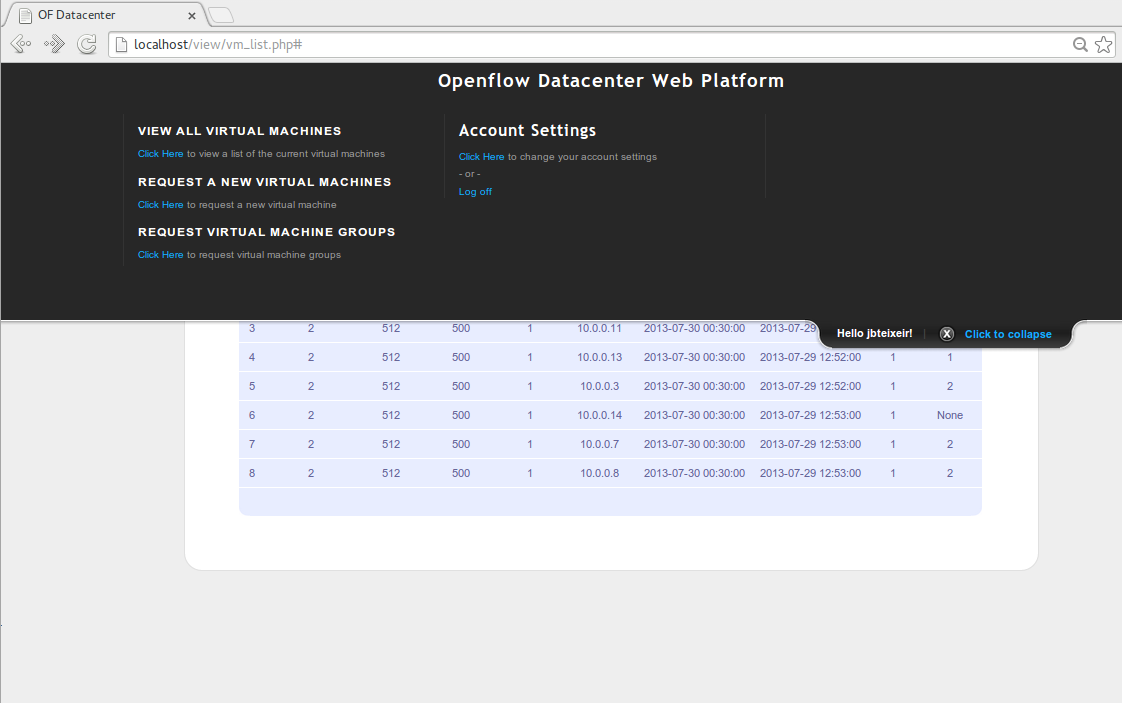
\includegraphics[width=1\textwidth]{figures/webplat_panel.png}
        \caption{Photo of the testing environment}
        \label{fig:realenv}
\end{figure}

\begin{figure}[htbp]
        \centering
        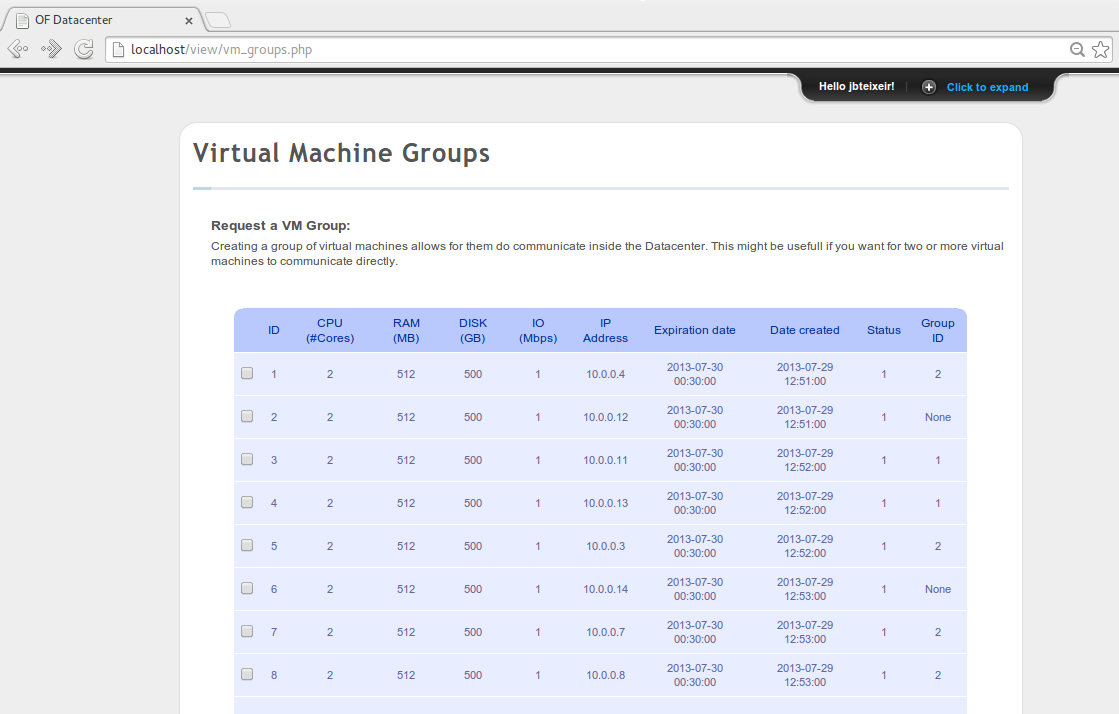
\includegraphics[width=1\textwidth]{figures/webplat_vmgroup.png}
        \caption{Photo of the testing environment}
        \label{fig:realenv}
\end{figure}

\begin{figure}[htbp]
        \centering
        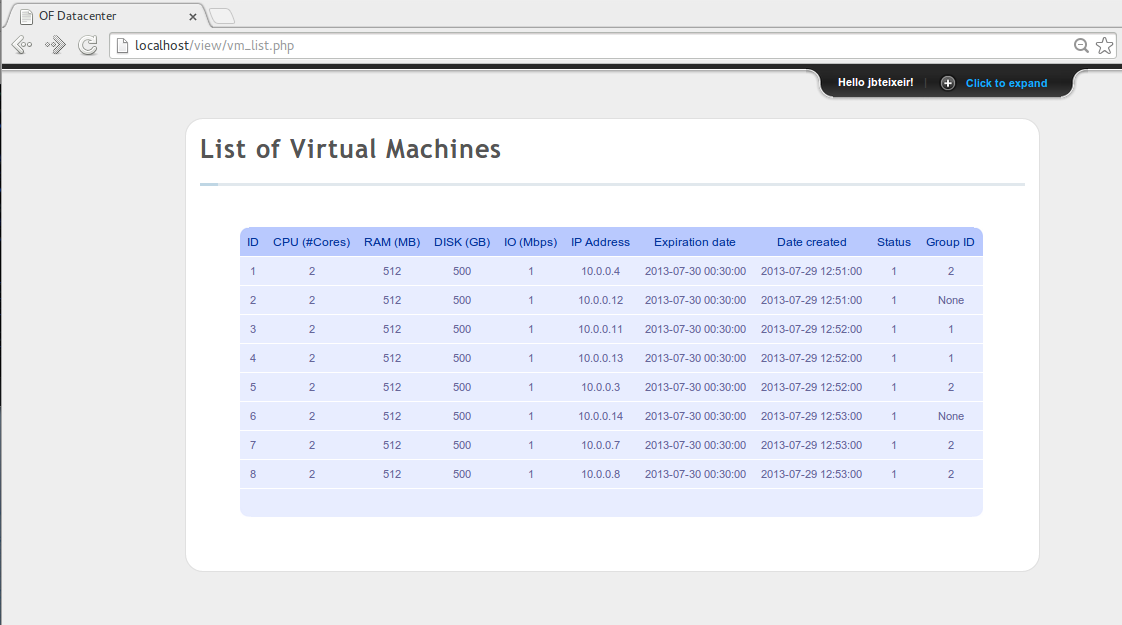
\includegraphics[width=1\textwidth]{figures/webplat_vmlist.png}
        \caption{Photo of the testing environment}
        \label{fig:realenv}
\end{figure}

\begin{figure}[htbp]
        \centering
        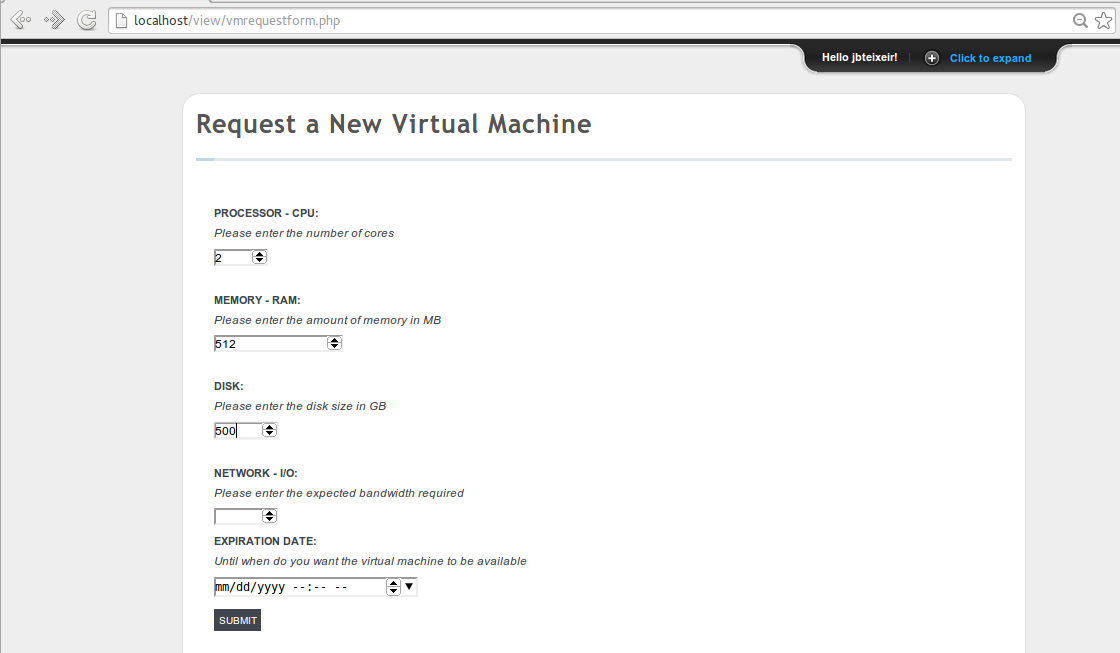
\includegraphics[width=1\textwidth]{figures/webplat_vmreq.png}
        \caption{Photo of the testing environment}
        \label{fig:realenv}
\end{figure}

Future work:
All the information in the database and both the controller access it
This would be good including for adding later monitoring (show statistics and everything - not only about the vm, but also about the switches (this last part just for the admin))
-basically add to the web platform a space where the admin/network engineer can interact with the controller without shutting it down change the code and run again (controller can be overrided in extreme cases - shutdown interfaces and stuff)


\newpage

\section{Framework modules: VM Requester}

As explained before, this modules is only to be used when testing.
Its purpose is to automatically generate VM requests.
In order to do so, it was used a poisson random variable, for both the interval between requests and the caracteristics of the request (CPU, RAM, DISK and IO). (When QoS was behing studied, the type of request was also variable according to the poisson random variable)
Its a simple python program that communicates with the controller VM request manager to send the request.
-threads were used for receiving the status of the VM request.
-show a print of it working

Future work:
-more random variables?

\newpage

\section{Using the framework}

\subsection{Emulator}

\subsubsection{Setting up the development environment}

Describe how to use the framework (emulation part) and how to access the API..

-add the photo

-add the specifications

-add image describing the structure

\subsection{Real Environment}

\subsubsection{Setting up the real environment}

-Figura com o esquema da configuração
Describe what changes in the real environment (the modules that are disabled and the ones that need to be enabled)

\begin{figure}[htbp]
        \centering
        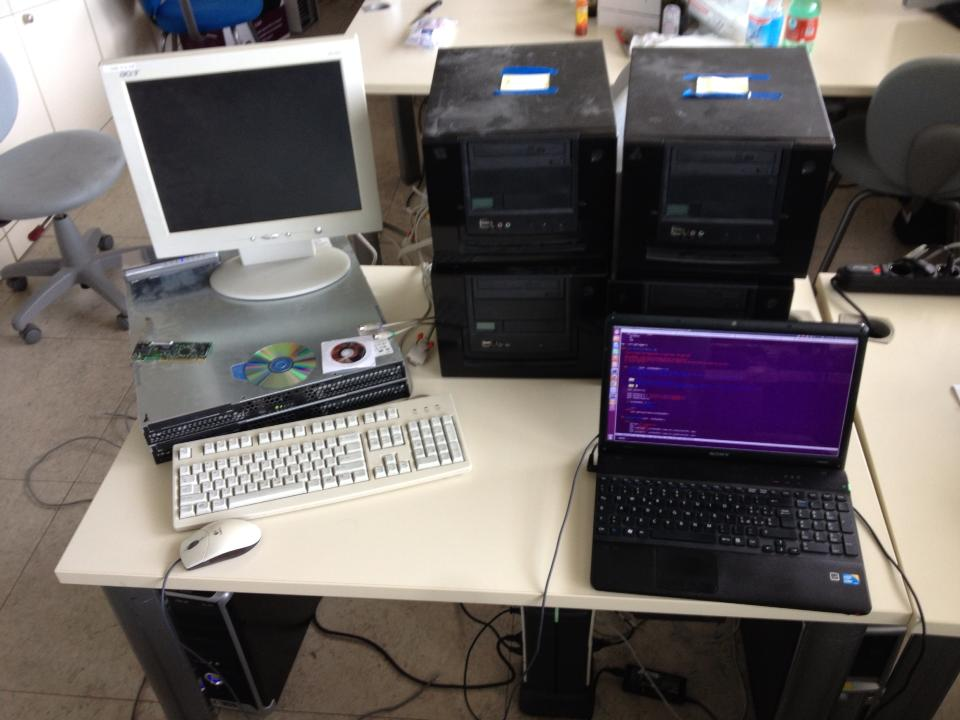
\includegraphics[width=0.7\textwidth]{figures/realenvironment.jpg}
        \caption{Photo of the testing environment}
        \label{fig:realenv}
\end{figure}

\begin{verbatim}
2 servers:

1 Intel Xeon CPU 3075@2.66Ghz
4 GB Ram
900 GB HD
NIC Intel 82566DM-2 Gigabit Network Connection
NIC Intel 82541GI Gigabit Network Connection

4 Mini-pc

1 AMD Phenom 9650 Quad-Core \@ 1.16Ghz

450 GB HD
4 GiB RAM
2 NIC Intel 82571EB Gigabit Ethernet Controller
1 NIC Realtek Semiconductor RTL8111/8168B Pci Express Gigabit Ethernet Controller
1 NetFPGA 4 ports Gigabit Ethernet

1 laptop

1 Intel Core i5 CPU M 480 \@ 2.67GHz x 4 
6 GiB RAM
250 GB HD
NIC Marvell Technology Group Ltd. Yukon Optima 88E8059 [PCIe Gigabit Ethernet Controller with AVB] (rev 11)

1 external machine

1 Intel Core i7 CPU 860 \@ 2.8Ghz x 8 
4 GiB Ram
450 GB HD
2 NIC 3com 3c905B 100BaseTX
1 NIC 3com 3c905C
1 NIC Realtek Semiconductor RTL8111/8168B Pci Express Gigabit Ethernet Controller

\end{verbatim}

\subsubsection{Real environment tests}
\begin{itemize}
  \item Talk about the environment which was setup
  \begin{itemize}
    \item Chosen hypervisor
    \item OpenVswitches VS NetFPGA problems
    \item 
  \end{itemize}
\end{itemize}

\newpage

\section{Framework extensions \label{Sec:fraext} }
\hspace{0.6cm}

Framework extensions were though to allow a wider range of experiments and to show that important subjects are been taken into consideration. QoS and VM migration were the two chosen, one from the network side and the other from the IT resources.
As most of the framework, the extensions are still a work-in-progress, thus they should only be seen as experiments.

\subsection{Enabling QoS}
\subsubsection{State of art: QoS in Openflow}
\hspace{0.6cm}

The OF protocol as been evolving to provide support for QoS.
However, as they argue that will bring extra complexity \cite{qosof}, until version 1.3.1 (latest) they only added support for simple queuing mechanisms.
Version 1.0 started by bringing to queues minimum guaranteed rate but queue configuration was still done outside the OF protocol. Later, in version 1.2, maximum rate was also included.

Although this features are available most research efforts focus on QoS approaches to OF using, among other techniques, dynamic routing and are oriented for either streamming\cite{ofqos2}\cite{ofqos3} or multimedia\cite{ofqos1}.

Regarding mininet and its OF switches implementation, the latest version is 2.0 and contains Open VSwitch driver 1.3.4, which fully supports OF 1.0.
More recent versions of OF can be integrated by upgrading the version of Open VSwitch, however, they are still experimental and may not include all the features provided in the protocol specification.

\subsubsection{QoS in the framework}
\hspace{0.6cm}

As the framework aims for providing the administrators/network engineers the tools for developing and testing their logic, it is their responsibility to develop QoS tecniques/algorithms similar to the ones shown previously, while the framework should limit itself to help with the interaction with the OF supported QoS features and their expected usage in the cloud DC.

However, as an experiment, we went for a different perspective on how QoS is used.
It was implemented traffic differentiation for giving different type of user, different types of QoE.
Instead of following the traffic classes, it was created classes of users/VM types (\textit{e.g.} free users vs gold users; VoIP server vs web server vs etc), where each queue corresponds to a class.

Bringing QoS into the framework implied making changes in all the main modules, mostly because it is associated with the requests, and, as said before, the current implementation of queues in OF switches must be done manually.
The following modules where modified:
\begin{itemize}
  \item \textbf{Mininet Environment} -- Added to \textit{Topology Generator} a method for creating for each port in each switch, the number of desired queues (classes) and their corresponding percentage of the whole bandwidth. It also takes into consideration the different link's bandwidth. \textit{Dpctl} was the tool used for creating the queues and \textit{tc} for setting the minimum rate.

  \item \textbf{VM Requests Generator} -- Attached to VM Requests the type of class. The type of the VM request is chosen by the already existing poisson random variable.

  \item \textbf{Controller}
  \begin{itemize}
    \item \textbf{VM Request Manager} -- Changed requests parsing and events thrown to include type of class.
    \item \textbf{Rules} -- Created new methods for installing the rules that will send the flows to the specific queues. The main difference for the previous method was the action used: ''openflowlib.ofp\_action\_enqueue(port = switch\_port, queue\_id = queue\_type))'', which included not only the port where the packets should be forwarded, but also the queue.

    \item \textbf{VM Allocation Manager} -- This was modified just for performing tests (this is were the desired logic would be implemented).Changed algorithms to allocate each VM type to a corresponding servers. This helps checking if the tests work, since the OF protocol does not have statistics for queues, only for ports.
  \end{itemize}
\end{itemize}

Figure \ref{fig:ofqos} shows a representation of the mininet topology and how it was possible to test the QoS solution.
It started by creating the shown topology and setting the links bandwidth equal for edge-to-server links and edge-to-aggregation links (so the bandwidth would have to be disputed and it was possible to see the queues in action).
By allocating two VMs of different types into two servers that share the same edge switch, and by setting their IO requirements to the maximum bandwidth capacity of the edge-to-aggregation link that they share (first green link counting from the bottom), it should be possible to see the class with more "minimum rate" have at least the bandwidth corresponding to its class.
The minimum rate configuration for the classes was 70\%-30\%.

Unfortunately, by analysing the ratios of the blue and red links, it was not possible to see any differentiation. Both servers got half of the available bandwidth - an output that was not expected.

\begin{figure}[h!tbp]
        \centering
        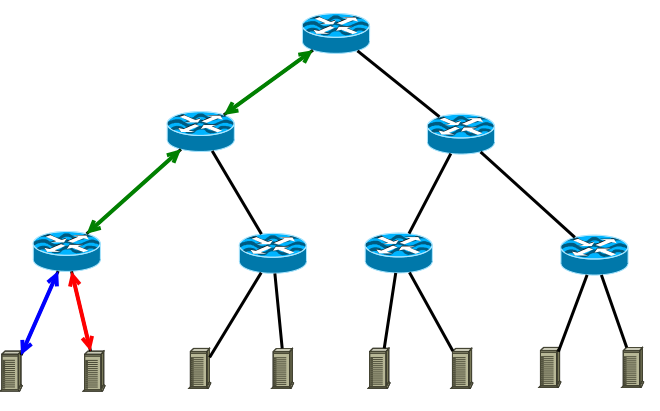
\includegraphics[width=0.8\textwidth]{figures/ofqos.png}
        \caption{QoS - Mininet testing environment}
        \label{fig:ofqos}
\end{figure}

A closer look to the article published online by the Openflow group\cite{qosof}, showed that the \textit{ENQUEUE} action was \textbf not supported yet, but that the queues could still be created and the flows could still be mapped to the queues by using the SET\_TOS and SET\_VLAN\_PCP OF parameters.
\begin{figure}[h!tbp]
        \centering
        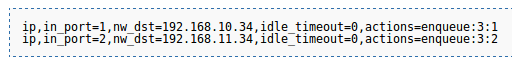
\includegraphics[width=0.8\textwidth]{figures/ofqosexample.png}
        \caption{QoS - Example of installed rules. Taken from \cite{qosof}}
        \label{fig:ofqosexample}
\end{figure}
As in their example they did not use any of these parameters, and the rules installed on the switches used the enqueue action (figure \ref{fig:ofqosexample}), the current implementation was misled.

\textit{Note: They have been contacted regarding how to reproduce such experiment, but no answer as been given yet.}

\newpage

\subsection{Enabling Virtual Machine migration}
\subsubsection{State of art: Virtual Machine migration}

VM migration is mostly handled by the hypervisors, which depending on the type of migration (live or not) take into consideration more or less requirements.
Research have been focus on helping making this tasks faster, simpler and without affecting the normal functioning of the DC.

More specifically, Stage A. et al. in \cite{vmmig1} discuss the management of bandwidth allocation while migrating VMs and also the assignment of priority to VM migration. They also propose an architecture design for DC.

Taking a step further, Boughzala, B. et al. \cite{vmmig2} used OF for supporting inter-domain VM migration. A study on how long rules take to be installed is made, and scalability is taken into consideration (usage of multiple OF controller, each with a specific OF domain). However it does not focus on helping VM migrations, only at allowing inter DCN migration.

By using OF rules to assist the Xen-based VM migration, Pedro S. Pisa et al \cite{vmmig3}, were able to have zero downtime. They also support WAN migration without packet loss due to the bilateral rule installation.

At last, Mishra, M. et al. in \cite{vmmig4}, present and overview of the VM migration techniques and how to use them to obtain dynamic resource management.
They point out the important characteristics of cloud-based DCs (Making resources available on demand, flexible resource provisioning and fine-grained metering), classify the resource management actions into types (server consolidation, load balancing and hotspot mitigation) and which heuristics are adopted (for each action) for answering when, which VM and where to migrate.

\subsubsection{Virtual Machine migration in the framework}

Aiming for providing full featured and generic access and control of the VM migration (being it live or not), a modified approach to the techniques previously presented was taken.

Although server consolidation and load balancing are the most used actions for resource management, they both fit in the same category - keeping DC policy.
Specially if we take into consideration the goal of the framework, it makes sense not to limit the resource management actions, but instead provide a generic way of keeping the DC policy, independently in what it is based (it might be server consolidation, but its up to the administrator/network engineer to define it).

\textit{Hotspot Mitigation} may also be split into server or network hotspot, which are quite different and have different ways of being solved.

Further more, since it is important to provide full access to DC, another question must be added -- which is the path chosen for VM migration.

For this to be possible, a few additions should be made to the controller:
\begin{itemize}
 \item Collect and save statistics from the servers.
 \item Add VM migration manager submodule to \textit{User-defined Logic}.
 \begin{itemize}
 \item \textit{When to migrate} -- Methods where it is defined how hotspots occurrence, for both network or server, are detected (or expected occurrence, so reactive and proactive VM migration are possible). Also a method for analyzing the current DC occupation (network and servers) and if it is not according to the defined policy (or combination of policies) start a VM migration process.
 \item \textit{Which VMs to migrate} -- Place for defining which VMs should be migrated.
 \item \textit{Where to migrate} -- Define where the VMs should be migrated.
 \item \textit{Which path to do the migration} -- Choose which path each migration should take.
 \end{itemize}
 Include methods for catching the hotspot raisen events where user defines what actions to take
\end{itemize}

\newpage
Although all the above should be defined by the administrator/network engineer, it would be an advantage if the \textit{keep DC policy} could be done automatically by using the already implemented policy in the \textit{user-defined logic}.

Having that in mind, the following algorithm was developed.\\

% \noindent\fbox{%
% \begin{varwidth}{\dimexpr\linewidth-2\fboxsep-2\fboxrule\relax}
\begin{algorithmic}[1]
\State {\textit{\%Retrive an ordered VM list (order can affect how many migration are needed)}}
\State {$vm\_list\gets getOrderedVmList()$}
\State {$vm\gets getVmFromList(vm\_list)$}
\While{$vm \neq null$}
\State {\textit{\%Get the server where the vm is allocated}}
\State {$vm\_place \gets getServer(vm)$}
\State {\textit{\%Subtract the current vm requirements to the server in which is allocated (to look like the vm was never allocated)}}
\State {$subtractVmToDC(vm)$}
\State {\textit{\%Run the user-defined policy to get the place where the vm should be allocated}}
\State {$new\_vm\_place \gets userDefinedAllocationPollicy(vm)$}
\If {$vm\_place \neq new\_vm\_place$}
\State {\textit{\%Get the migration path for this vm}}
\State {$vm\_migration\_path \gets getVmMigrationPath(vm\_place, new\_vm\_place)$}
\State {\textit{\%Start the vm migration}}
\State {$migrateVM(vm, vm\_place, new\_vm\_place, vm\_migration\_path)$}
\EndIf
\State {$vm\gets getVmFromList(vm\_list)$}
\EndWhile

\end{algorithmic}
% \end{varwidth}% 
% }
        
\begin{verbatim}


\end{verbatim}
-independently of being live or non live migration
-say a diferent view can be applyed, a wider one.
-explain how it was though to be used in the framework, and which where the goals
-make a pseudo code about the ''keeping the DC policy''

\subsubsection{Example}

Give two examples with best and worst fit
images with steps is a good idea (images side by side)

\chapter{Validation and tests \label{cha:valtes} }

Usually test and validation of the proposed solution ...

\section{Framework Validation}

Understanding the impact on the DC network infrastructure of well--known VM allocation policies represents the first step for finding more and more optimized solutions. Our main concern was to validate our framework analyzing the behaviour of the system under common situations, in order to compare the obtained results with the theoretical ones. For this reason in the \textit{user-defined logic} part of the controller, we firstly implemented Best Fit (BF), then Worst Fit (WF). The BF algorithm chooses the server with the smallest available resources that still suits the requirements. On the other hand WF chooses the one with the most available resources. Therefore, we expected that as each request comes, using a BF policy, all the VMs should be allocated in one single host until it is able to fulfill the requirements. Then a new host will be selected, and so on until all the hosts have no more free space. In the second case (\textit{i.e.}, WF policy), the VMs should be firstly equally spread through all 
the hosts. We configured the DC topology with $1$ outside host, $2$ core switches, $4$ aggregation switches, $8$ edge switches, and $16$ hosts (\textit{i.e.}, $2$ per edge). We set each host to be able to allocate up to $3$ VM, for sake of simplicity (and to easily understand the results), and all the requests equal in terms of requirements (\textit{i.e.}, CPU, RAM, amount of disk space and bandwidth). We defined the host link ratio as the amount of traffic received per host against the link speed set on the DC initialization phase. We also set the DC in order to saturate the host link when three different VMs have been allocated.

\begin{figure}[h!tbp]
        \centering
        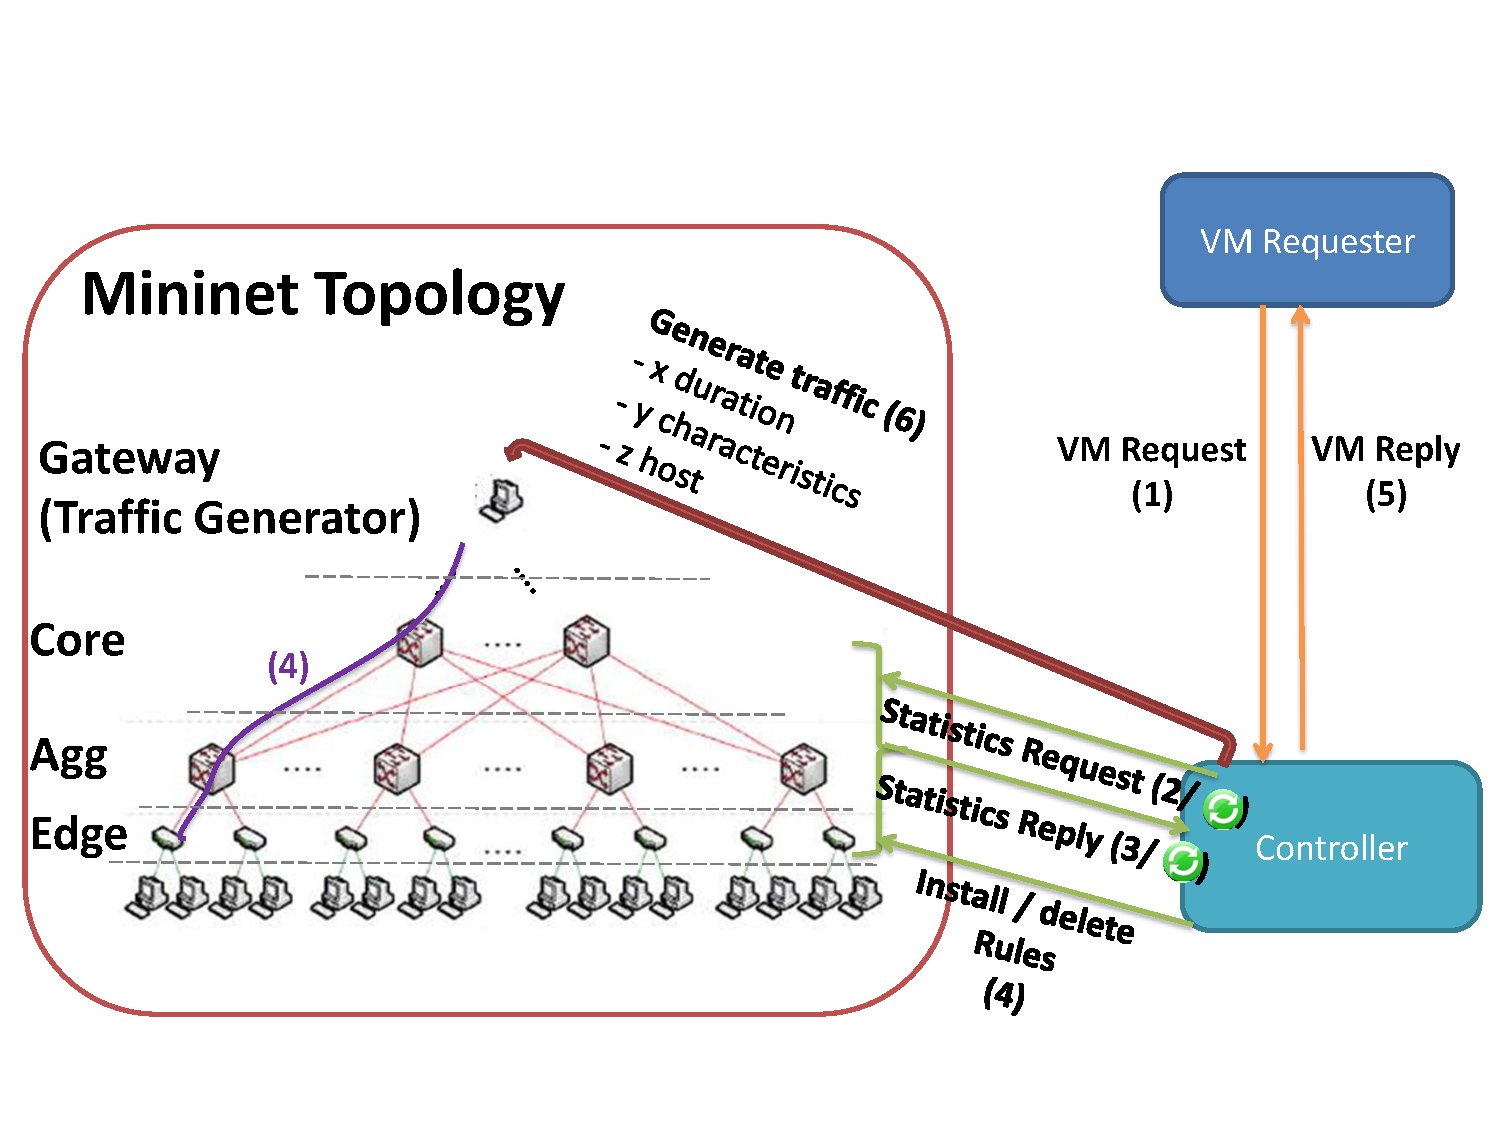
\includegraphics[width=0.45\textwidth]{figures/figure1.pdf}
        \caption{The environment}
        \label{fig:use_case}
\end{figure}


Figure \ref{fig:use_case} shows an high--level vision of the proposed environment. Starting from our framework, we only added few lines of code to implement the allocation policy, since it provides all the necessary APIs to make sure that the controller can interact with the VM Requester, Traffic Generator and the DC switches. Every time the controller receives a new VM allocation request (\textit{i.e.}, generated by the VM requester according to the DC configuration) it installs the proper rules on the switches (optionally it can ask for switches statistics -- even periodically). Once this process is completed, the controller informs the VM requester about the result of the allocation process and the traffic generation starts.


\begin{figure}[h!tbp]
        \centering
        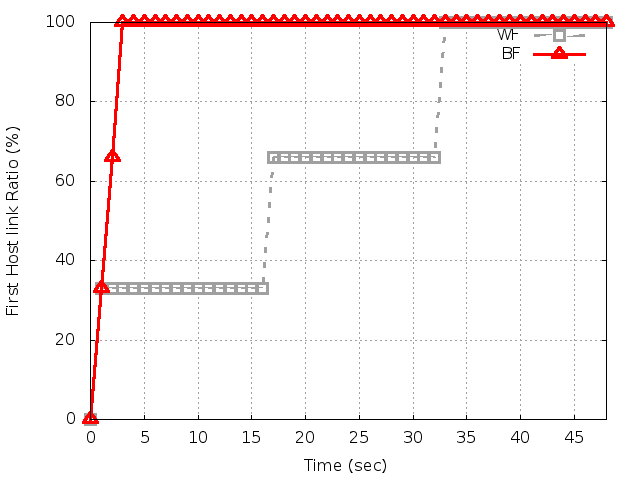
\includegraphics[width=0.6\textwidth]{figures/use_case.png}
        \caption{WF vs BF}
        \label{fig:wf_bf}
\end{figure}

Figure \ref{fig:wf_bf} shows the first host link ratio over the time. Using a BF allocation policy, once a VM has been allocated in a host, all the following VMs are allocated in the same host until no more could be allocated (\textit{e.g.}, useful for energy saving). Having a new VM allocation request per second, after three seconds the first host link reaches the saturation. Using the WF policy instead, the VMs should be firstly equally spread through all the hosts. In fact, being $16$ the DC hosts, and having just $1$ request per second, the first host link saturate at the $33$--th second.


\begin{itemize}
	\item Show how Bf goes against WF with server driven algorithm (show server occupation)
	\item Show how Bf goes against WF with network driven algorithm (show network occupation) (although the behaviour is similar is allow to say that net algorithm may use switch statistics)
\end{itemize}
\newpage


\section{Performance Evaluation}
\label{sec:perf}
\hspace{0.6cm}

TODO: CHANGE THIS FOR NOT BEING IN THE SECOND PERSON OF THE PLURAL
TODO: PUT IMAGES IN THE RIGHT PLACE (ALONG WITH THE TEXT)

We evaluated the actual performance of the proposed framework through a variety of experiments using a PC equipped with an Intel i5 3GHz and 8GB of DD3 RAM (\textit{i.e.}, from now on we will call it Host-PC).
The first tests have been carried out to inspect the impact of the amount of generated traffic, the DC topology size and the number of outside hosts on the host link ratio.
Firstly, we generate a static topology (\textit{i.e}, $2$ outside hosts, $2$ core switches, $4$ aggregation switches, $8$ edge switches, $8$ hosts), then we started measuring the host link ratio increasing the generated traffic per host.

\begin{figure}[h!tbp]
        \centering
        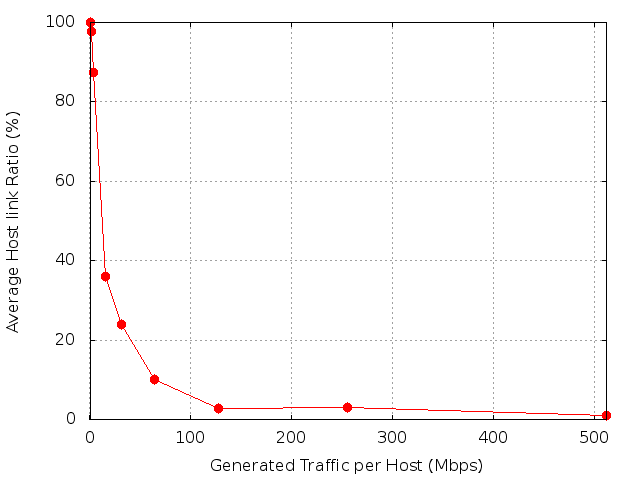
\includegraphics[width=0.7\textwidth]{figures/bw_utilization.png}
        \caption{Average Host link Ratio vs per Host Generated Traffic}
        \label{fig:bw}
\end{figure}

As shown in figure \ref{fig:bw} we were able to generate up to few Mbps of traffic per host.
Then the host link ratio decreases as the generated traffic grows.
We point out that such limitation does not affect any kind of DC performance tests made with our framework,
because we can scale the link speed as much as we want during the DC initialization phase, reaching every time 100\% of host link ratio.

In order to test the impact of the DC topology size on the
host link ratio we kept the amount of the generated aggregated traffic 
constant while exponentially increasing the number of switches and hosts.
We started from the previous test topology.

On DC initialization phase, we set the link speed in order to fully saturate the host links.

\begin{figure}[h!tbp]
        \centering
        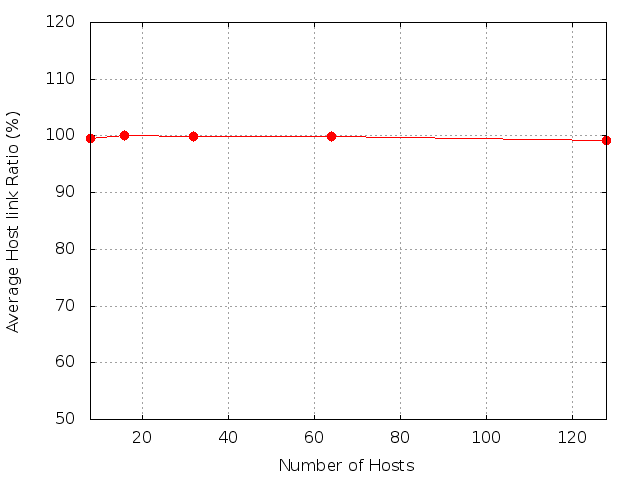
\includegraphics[width=0.7\textwidth]{figures/topo.png}
        \caption{Average Host Link Ratio vs number of Hosts}
        \label{fig:topo}
\end{figure}

The results in figure \ref{fig:topo} show that regardless of the hosts number, the host link ratio remains constant.
This means that as long as the total amount of generated traffic per host and the links speed can guarantee the link saturation, the system can scale indefinitely, being the only limits the Mininet itself, or the controller. 
Finally we investigated the relationship between the number of hosts connected to just one outside host and the average link ratio.

\newpage

\begin{figure}[h!tbp]
        \centering
        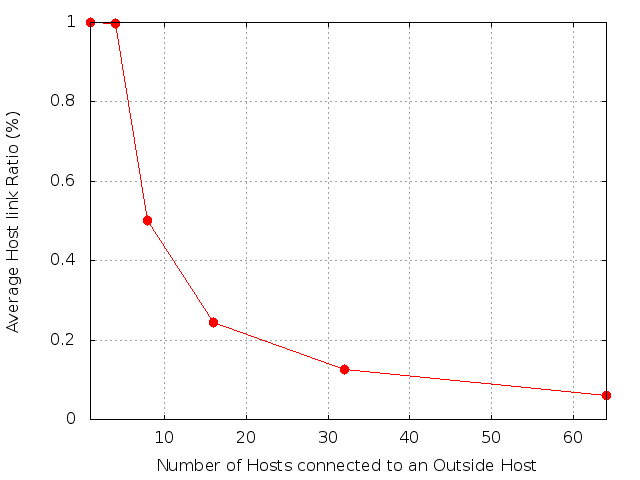
\includegraphics[width=0.7\textwidth]{figures/out_hosts_ratio.png}
        \caption{Average Host Link Ratio vs number of Hosts per Outside Host}
        \label{fig:hosts}
\end{figure}

Figure \ref{fig:hosts} shows that a maximum of $8$ hosts can be managed by just one outside host (\textit{i.e.}, the host link speed is set in order to have a link saturation).

Such a result gives to the user an important constraint that should be used during the DC configuration phase.
We point out that this limitation is native of the Mininet environment and it is not due to our framework.
The second tests have been carried out to inspect the impact of both the amount of generated traffic and the DC topology size on the amount of memory the Host-PC needs.

\newpage

\begin{figure}[h!tbp]
        \centering
        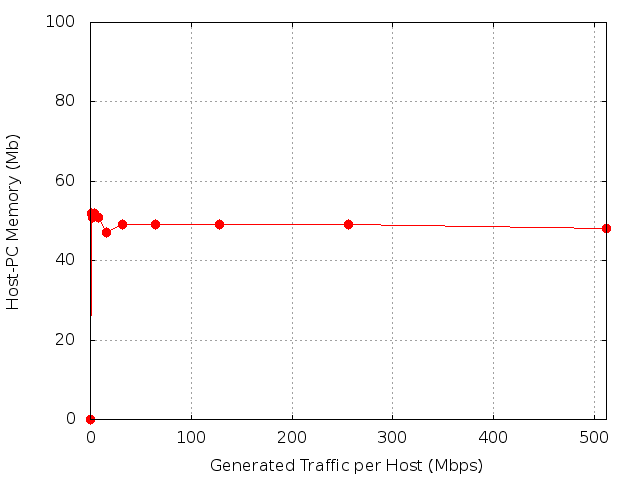
\includegraphics[width=0.7\textwidth]{figures/mem1_utilization.png}
        \caption{Host-PC Memory Utilization vs per Host Traffic Generated}
        \label{fig:mem1}
\end{figure}

\begin{figure}[h!tbp]
        \centering
        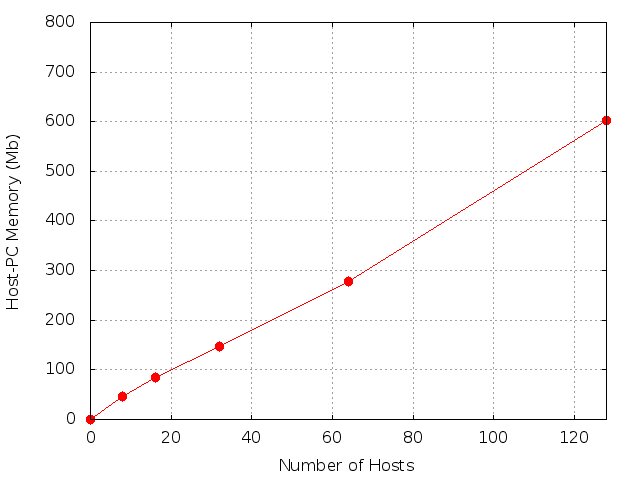
\includegraphics[width=0.7\textwidth]{figures/mem2_utilization.png}
        \caption{Host-PC Memory Utilization vs number of Hosts}
        \label{fig:mem2}
\end{figure}

Figure \ref{fig:mem1} shows that the memory utilization does not depend on the amount of generated traffic for each host.
On the other hand, as shown in figure \ref{fig:mem2}, as the topology size grows, the memory usage also grows in the same proportion, which allows to conclude that it scales linearly.
\newpage

\chapter{Conclusions\label{cha:conclusions}}

This chapter provides ...

\section{Main contributions}

\section{Future work}

\appendix

\chapter{Mininet Environment -- Configuration File\label{app:minconf}}

\begin{verbatim}
Filename: conf.ini

[TopologySwitches]
#Integer value
#core_no - number of core switches
#agg_no - number of aggregation switches
#edge_no - number of edge switches
core_no = 4
agg_no = 8
edge_no = 16

[TopologyHosts]
#Integer value
#out_no - number of outside hosts
#host_no - number of hosts per edge switch
#host_detectacle_time - time in seconds in which the hosts send packets 
# so the host_tracker can detect them (0 == always detectable)
out_no = 4
host_no = 2
host_detectable_time = 2

[TopologyLinks]
#Integer value
#edgetoagglinkno - number of links that connect each edge switch to 
# aggregation switches
#aggtocorelinkno - number of links that connect each aggregation switch 
# to core switches
#coretooutlinkno - number of links that connect each core switch to 
# outside hosts
edgetoagglinkno = 2
aggtocorelinkno = 2
coretooutlinkno = 1

[SwitchBandwidth]
#Float value - mbps
#out_bw - bandwitdh for links that connect outside hosts
#core_bw - bandwitdh for links that connect core switches
#agg_bw - bandwitdh for links that connect aggregation switches
#edge_bw - bandwitdh for links that connect edge switches
out_bw = 4
core_bw = 4
agg_bw = 2
edge_bw = 1

[SwitchQueues]
#Float value
#queue_no - number of queues per switch and per port
#queue_number = bandwidth ratio - queue minimum bandwidth 
# (please use lower numbers for higher priority so the controller can assign premium users to this queues)  
queue_no = 2
queue_bw1 = 0.8
queue_bw2 = 0.2

[Traffic]
#Iperf configuration
#Amount of udp traffic against tcp one
#starting port for iperf to run on each host
udp_ratio = 0.5
iperf_port = 16000

[Socket]
#path for the unix socket
socket_path = /home/mininet/socket.tmp

\end{verbatim}

\cleardoublepage

\markright{\slshape Appendix}

\cleardoublepage
\bibliographystyle{unsrt}
\addcontentsline{toc}{chapter}{\bibname}

%% Add file.bib
\bibliography{sigproc}
\nocite{*}



\end{document}

%Layout do Vasco
% 0- Resumo/abstract
% 1- Conceitos Introdutórios
% WebRTC (APIs W3C)x, ICEx/STUNx/TURNx, RTP/DTLSx, Codecs, Protocolos DataChannel (UDP - SCTPx - DTLSx), Sinalização (draft JSEP, SIP sobre WebSockets, Jingle sobre WebSockets), WebSockets
% 2- Estado da Arte
% soluções existentes:
% Libs javascript incl as Libs do Muaz
% Sinalização: node.js, vertx
% Gateways para SIP
% 3- Requisitos e Casos de Uso
% 4- Experimentação e Seleção de Soluções Existentes
% Node.js vs Vertx
% Libs do Muaz vs ?
% 5- Arquitectura e Desenho
% Especificação das APIs Javascript e do Servidor (manual para programador)
% 6- Validação e Testes
% Aplicação 
% 7- Conclusões